\documentclass[a4paper,12pt]{article}
\usepackage{czech}                    
\usepackage[utf8]{inputenc}         
\usepackage{a4wide}                   
\usepackage[pdftex]{graphicx}        
\usepackage{graphics}
\usepackage{indentfirst}   
\usepackage{fancyhdr}                 
\usepackage{setspace}
\usepackage{amsmath}
\usepackage{amssymb}
\usepackage{epsfig}

%%\usepackage{nopageno}
%%\usepackage{txfonts}
\usepackage[usenames]{color}

\begin{document}
% \input epsf 
\section{Úkol}
\begin{enumerate}
	\item Změřte dobu kmitu $T_0$ dvou stejných nezávislých fyzických kyvadel.
	\item Změřte dobu kmitů $T_i$ dvou stejných fyzických kyvadel vázaných slabou pružnou vazbou vypouštěných z klidu při počátečních podmínkách:
	\begin{enumerate}
		\item	$y_1=y_2=B$ ... doba kmitu $T_1$
		\item $y_1=-y_2= B$ ... doba kmitu $T_2$
		\item $y_1=0, y_2= B$
		\begin{enumerate}
			\item doba kmitu $T_3$
			\item doba $T_4/4$, za kterou dojde k maximální výměně energie mezi kyvadly 
		\end{enumerate}
	\end{enumerate}
	\item Vypočtěte kruhové frekvence $\omega_0$, $\omega_1$, $\omega_2$, $\omega_3$ a $\omega_4$ odpovídající dobám $T_0$, $T_1$, $T_2$, $T_3$ a $T_4$, ověřte měřením platnost vztahů odvozených pro $\omega_3$ a $\omega_4$.
	\item Vypočtěte stupeň vazby $\kappa$.
	\item Pro jednu pružinu změřte závislost stupně vazby na vzdálenosti zavěšení pružiny od uložení závěsu kyvadla a graficky znázorněte. 
\end{enumerate}

\section{Teorie}
\noindent
Vázané scilátory jsou v našem případě dvě identická kyvadla, mezi kterými je upevněna ve vzdálenosti $d$ od osy otáčení pružina. Pro každé z nich platí
\begin{eqnarray}
	T=\sqrt{{D \over J}},
\end{eqnarray}
kde $D$ je direkční moment a $J$ moment setrvačnosti kyvadla. Pro samostatné kyvadlo též platí
\begin{eqnarray}
	M=\alpha D,
\end{eqnarray}
kde $M$ je moment síly potřebný k vychýlení osy kyvadla o úhel $\alpha$. Při zapojení pružiny se začne projevovat její vlastní direkční moment $D^*$, který je závislý na tuhosti pružiny a vzdálenosti $d$ uvedené výše.

V závislosti na počátečních podmínkách tyto kyvadla splňují význačné pohybové rovnice. Obecnější řešení naleznete v \cite{1}. První případ je $y_1(0)=y_2(0)=A, \dot y_1(0)=\dot y_2(0)=0,$ kde $y_i$ jsou výchylky kyvadel. V tomto případě splňují kyvadla rovnici
\begin{eqnarray}
	\varphi_1=\varphi_2=A\cos \omega_1,
\end{eqnarray}
kde $A$ je maximální amplituda a
\begin{eqnarray}
	\omega_1=\sqrt{{D\over J}}.
\end{eqnarray}
Pro druhý případ jsou počáteční podmínky $y_1(0)=-y_2(0)=B, \dot y_1(0)=\dot y_2(0)=0$, při kterých splňují rovnici
\begin{eqnarray}
	\varphi_1=-\varphi_2=A\cos \omega_2,
\end{eqnarray}
kde $A$ je amplituda a 
\begin{eqnarray}
	\omega_2=\sqrt{{D+2D^* \over J}}.
\end{eqnarray}
Z těchto dvou případů se dá dopočítat případ $y_1(0) ,y_2(0)=B, \dot y_1(0)=\dot y_2(0)=0$, pro který platí
\begin{eqnarray}
	\varphi_1=A\sin\left[{1\over 2}(\omega_2-\omega_1)t\right]\cos\left[{1\over 2}(\omega_2+\omega_1)t\right], \\
	\varphi_2=A\cos\left[{1\over 2}(\omega_2-\omega_1)t\right]\sin\left[{1\over 2}(\omega_2+\omega_1)t\right]
\end{eqnarray}

Při slabé vazbě můžeme rovnice (7), (8) interpretovat tak, že obě kyvadla kmitají se stejnou frekvencí
\begin{eqnarray}
	\omega_3={1 \over 2}(\omega_2+\omega_1)
\end{eqnarray}
a jejich ampitudy se periodicky mění s frekvencí
\begin{eqnarray}
	\omega_4={1 \over 2}(\omega_2-\omega_1).
\end{eqnarray}

Tyto frekvence zjistíme naměřením času $t$, za který kyvadlo vykoná $n$ kmitů a dosazením do rovnice
\begin{eqnarray}
	\omega={2\pi n \over t}.
\end{eqnarray}

Výsledný vztah pro výpočet stupňe vazby je dle \cite{1}
\begin{eqnarray}
	\kappa={\omega_2^2-\omega_1^2 \over \omega_2^2+\omega_1^2}.
\end{eqnarray}

Podrobnější rozbor mechaniky kyvadel naleznete v \cite{2} 

K měření byli k dispozici dvě pružiny různé tuhosti, stopky, metr a kyvadla. 

\section{Výsledky měření}
\noindent
Vnější podmínky nemély žádné důsledky na přenost měření, tudíž je neuvádím.

\subsection{Stupeň vazby}
\noindent
Nejprve jsem nastavil háčky na uchycení pružiny u obou kyvadlech do stejné vzdálenosti od osy otáčení a změřil ji. Hodnoty naleznete v tabulce 1.
$$
\begin{array}{|l|cccccccccc|}
\hline
	d_0/\mbox{cm} &34.6&34.5&34.6&34.5&34.4&34.4&34.5& 34.5& 34.4& 34.6\\ \hline
\end{array}
$$
\begin{center}
	\vglue0.05in
	\textbf{Tabulka 1:} Vzdálenost úchytů od osy otáčení
\end{center} 
Následně jsem ověřil, zda jsou obě kyvadla dobře zkalibrovaná, a to tak, že jsem změřil dobu deseti kmitů každého z kyvadel, které jsou shrnuty v tabulce 2 pod označením $T_0^1$ a $T_0^2$, a dle vztahu (11) stanovil jejich periody spolu s jejich chybami dle \cite{4}
\begin{eqnarray}
T_0^1=(1.91\pm 0.01)\mbox{s}, \\
T_0^2=(1.91\pm 0.01)\mbox{s}
\end{eqnarray}
\begin{displaymath}
\begin{array}{|c|c|c|}
\hline
	n&10\cdot T_0^1/\mbox{s} & 10\cdot T_0^2/\mbox{s} \\ \hline
	1 & 19.07 &19.05 \\ \hline
	2 & 19.04 & 19.13 \\ \hline
	3 & 19.14 & 19.09 \\ \hline
	4 & 18.98 & 19.05 \\ \hline
	5 & 19.05 & 19.02 \\ \hline
\end{array}
\end{displaymath}
\begin{center}
	\vglue0.05in
	\textbf{Tabulka 2:} Doba deseti kmitů jednotlivkých kyvadel.
\end{center}

Poté jsem postupně zavěšoval na háčky pružiny a měřil výzačné připady popsané výše. Dále v textu je vždy příslušný případ ozačen dolním indexem a horní značí typ pružiny. Z těchto naměřených hodnot jsem dle \cite{4} stanovil jejich střední hodnotu a chybu. Měření jsou shrnuta v tabulkách 3,4,5 a 6.

$$
\begin{array}{|c|c|c|c|c|c|}
\hline
	n&	10\cdot T_1^1/\mbox{s}&	10\cdot T_1^2/\mbox{s}&	n&	10\cdot T_1^1/\mbox{s}&	10\cdot T_1^2/\mbox{s} \\ \hline	
	1&	19.09&	19.04&	6&	19.08&	19.06 \\ \hline
	2&	19.15&	19.05&	7&	19.10&	19.09 \\ \hline
	3&	19.02&	19.02&	8&	19.04&	19.08 \\ \hline
	4&	19.05&	19.01&	9&	19.05&	19.05 \\ \hline
	5&	19.08&	19.04&	10&	19.06&	19.02 \\ \hline
\end{array}
$$
\begin{center}
	\vglue0.05in
	\textbf{Tabulka 3:} Doba deseti period pro případ stejné výchylky na obou kyvadlech.
\end{center}

$$
\begin{array}{|c|c|c|c|c|c|}
\hline
	n&	10\cdot T_2^1/\mbox{s}&	10\cdot T_2^2/\mbox{s}&	n&	10\cdot T_2^1/\mbox{s}&	10\cdot T_2^2/\mbox{s} \\ \hline	
	1&	18.24&	16.88&	6&	18.22&	16.89 \\ \hline
	2&	18.18&	16.89&	7&	18.14&	16.92 \\ \hline
	3&	18.22&	16.89&	8&	18.20&	16.79 \\ \hline
	4&	18.29&	16.89&	9&	18.21&	16.95 \\ \hline
	5&	18.22&	16.85&	10&	18.15&	16.89 \\ \hline
\end{array}
$$
\begin{center}
	\vglue0.05in
	\textbf{Tabulka 4:} Doba deseti period pro případ opačné výchylky na kyvadlech.
\end{center}

$$
\begin{array}{|c|c|c|c|c|c|}
\hline
	n&	7\cdot T_3^1/\mbox{s}&	3\cdot T_3^2/\mbox{s}&	n&	7\cdot T_3^1/\mbox{s}&	3\cdot T_3^2/\mbox{s} \\ \hline	
	1&	12.93&	5.18&	6&	12.93&	5.27 \\ \hline
	2&	12.88&	5.44&	7&	12.94&	5.37 \\ \hline
	3&	13.00&	5.31&	8&	13.06&	5.35 \\ \hline
	4&	12.98&	5.34&	9&	12.89&	5.36 \\ \hline
	5&	12.99&	5.35&	10&	12.96&	5.39 \\ \hline
\end{array}
$$
\begin{center}
	\vglue0.05in
	\textbf{Tabulka 5:} Doba sedmi respektive tří period pro případ vychýlení jednoho kyvadla.
\end{center}

$$
\begin{array}{|c|c|c|c|c|c|}
\hline
	n&	{1 \over2}\cdot T_4^1/\mbox{s}&	{1 \over 2}\cdot T_4^2/\mbox{s}&	n&	{1\over2}\cdot T_4^1/\mbox{s}&	{1\over2}\cdot T_4^1/\mbox{s} \\ \hline	
	1&	39.79&	14.03&	6&	40.23&	14.14 \\ \hline
	2&	39.92&	13.95&	7&	40.99&	14.09 \\ \hline
	3&	39.60&	14.66&	8&	39.89&	14.62 \\ \hline
	4&	38.99&	13.81&	9&	39.77&	14.82 \\ \hline
	5&	40.18&	13.90&	10&	39.83&	14.36 \\ \hline
\end{array}
$$
\begin{center}
	\vglue0.05in
	\textbf{Tabulka 6:} Doba, za kterou se druhé kyvadlo opět zastaví, pokud vychýlíme pouze první.
\end{center}

Po jejich vyhodnocení dle \cite{4} mi vyšli výsledné doby period
\begin{eqnarray}
	T_1^1&=&(1.91 \pm 0.01) \mbox{s} \\
	T_2^1&=&(1.82 \pm 0.01) \mbox{s} \\
	T_3^1&=&(1.85 \pm 0.01) \mbox{s} \\
	T_4^1&=&(79.8 \pm 0.7) \mbox{s} \\
	T_1^2&=&(1.90 \pm 0.01) \mbox{s} \\
	T_2^2&=&(1.69 \pm 0.01) \mbox{s} \\
	T_3^2&=&(1.78 \pm 0.03) \mbox{s} \\
	T_4^2&=&(28.6 \pm 0.6) \mbox{s}
\end{eqnarray}

Dle (11) a vzorců pro přenos chyby z \cite{4} jsem dopočetl výsledné frekvence
\begin{eqnarray}
	\omega_1^1&=&(3.29 \pm 0.03) \mbox{s} \\
	\omega_2^1&=&(3.45 \pm 0.02) \mbox{s} \\
	\omega_3^1&=&(3.40 \pm 0.02) \mbox{s} \\
	\omega_4^1&=&(7.87 \pm 0.07)\cdot 10^{-2} \mbox{s} \\
	\omega_1^2&=&(3.31 \pm 0.02) \mbox{s} \\
	\omega_2^2&=&(3.72 \pm 0.02) \mbox{s} \\
	\omega_3^2&=&(3.53 \pm 0.02) \mbox{s} \\
	\omega_4^2&=&(2.20 \pm 0.05)\cdot 10^{-1} \mbox{s}
\end{eqnarray}

Po dosazení do rovnic (9) a (10) jsem zjistil, že mnou naměřené hodnouty $\omega_3$ a $\omega_4$ odpovídají v rámci chyby měření těm vypočteným.

Nakonec jsem dle (12) vypočetl stupeň vyzby pro jednotlivé pružiny
\begin{eqnarray}
	\kappa^1=(4.74\pm0.07)\cdot 10^{-2}, \\
	\kappa^2=(1.16\pm0.02)\cdot 10^{-1}
\end{eqnarray}

\subsection{Závislost $\kappa$ na poloze pružiny}
\noindent
Pro lepší viditelnost závislosti jsem zvolil pružinu s vyšším stupněm vazby. Počátek souřadnice $d$ jsm si položil do nejvyššího místa, kam se dal háček na pružinu umístit. Vycházel jsem z předpokladu, že perioda $T_1$ dle značení výše nezávisí na $\kappa$, což jsem si ověřil pro krajní hodnoty, a tak jsem měřil pouze $T_2$ pro jednotlivé hodnoty $d$. Naměřené hodnoty jsou spolu s výslednou periodou a stupněm vazby včetně chyby v tabulce 7.
$$
\begin{array}{|c|ccccc|c||c|}
\hline
	d/\mbox{cm}&	\multicolumn{5}{|c|}{10\cdot T^i_2/\mbox{s}} & T_2/\mbox{s}& \kappa \\ \hline
	0&19.07&19.08&19.14&19.02&19.07&1.91\pm 0.01&	0.00\pm 0.0001 \\ \hline
	9&	18.67&	18.74&	18.82&	18.73&	18.73&1.87\pm 0.01&	0.0211\pm0.0003\\ \hline
	18&	18.21&	18.13&	18.11&	18.08&	18.07&1.81\pm 0.01&	0.0532\pm0.0008\\ \hline
	27&	17.49&	17.54&	17.45&	17.47&	17.51&1.75\pm 0.01&	0.087\pm0.001\\ \hline
	36&	16.83&	16.81&	16.75&	16.68&	16.74&1.68\pm 0.01&	0.128\pm0.002\\ \hline
	45&	16.21&	16.12&	16.16&	16.08&	16.09&1.61\pm 0.01&	0.168\pm0.002\\ \hline
\end{array}
$$
\begin{center}
	\vglue.05in
	\textbf{Tabulka 7:} Závislost stupně vazby na vzdálenosti pružiny od osy otáčení.
\end{center}	
Tuto závislost jsem zanesl do grafu 1 a pro lepší názornost proložil parabolou.
\begin{center}
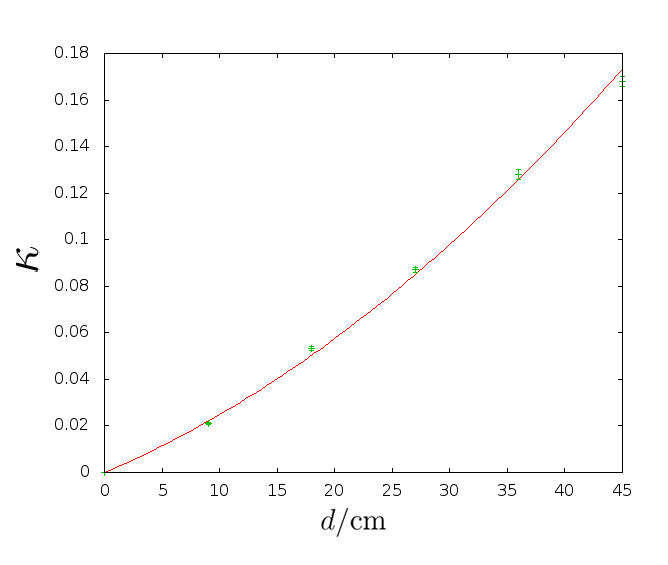
\includegraphics[width=5in]{graf1.png}
\vglue.05in
\textbf{Graf 1:}Závislost stupně vazby na vzdálenosti pružiny od osy otáčení.
\end{center}

\section{Diskuze}
\noindent 
Přesnost měření $T_1$ a $T_2$ dále potřebných pro výpočet $\kappa$ byla vysoká, a proto si myslím, že výsledek odpovídá skutečnosti. S ostatnímy časy se již vyskytovaly nemalé potíže. Zaprvé u periody $T_3$ jsem musel snížit počet kmitů, které jsem počítal, protože okolo nulové výchylky nebylo možné stanovit jejich počet. Tím se samozřejmě výrazně zvýšila chyba daná především reakční dobou, obzvláště u tužší pružiny, kdy jsem byl schopen přesně určit pouze 3 kmity. U periody $T_4$ nastal problém s přesným určením doby, kdy se druhé kyvadlo opět zastavilo, protože nebylo mnohdy poznat, jestli už se tak stalo, či nikoliv. U tohoto měření je také chyba zdaleka největší, protože jsem tento fakt musel vzít v úvahu ve statistické chybě. I přes tyto nepřesnosti se všask ukázalo, že vzorce (11) a (12) jsou správné.
Díky tomu, že k závilosti $\kappa$ na vzdálenosti pružiny od osy otáčení bylo zapotřebí pouze prvních dvou period je výsledná chyba opět minimální a z grafu je dobře vidět, že se nejedá o lineární závislost.


\section{Závěr}
\noindent
Změřil jsem periodu dvou nezávislých fyzických kyvadel
\begin{eqnarray}
T_0^1=(1.91\pm 0.01)\mbox{s}, \\
T_0^2=(1.91\pm 0.01)\mbox{s}.
\end{eqnarray}
Změřil jsem periody vázaných kyvadel $T_i$ při počátečbích podmínkách dle zadání
\begin{eqnarray}
	T_1^1&=&(1.91 \pm 0.01) \mbox{s}, \\
	T_2^1&=&(1.82 \pm 0.01) \mbox{s}, \\
	T_3^1&=&(1.85 \pm 0.01) \mbox{s}, \\
	T_4^1&=&(79.8 \pm 0.7) \mbox{s}, \\
	T_1^2&=&(1.90 \pm 0.01) \mbox{s}, \\
	T_2^2&=&(1.69 \pm 0.01) \mbox{s}, \\
	T_3^2&=&(1.78 \pm 0.03) \mbox{s}, \\
	T_4^2&=&(28.6 \pm 0.6) \mbox{s}.
\end{eqnarray}
Vypočetl jsem frekvence $\omega_i$ odpovídající periodám výše
\begin{eqnarray}
	\omega_1^1&=&(3.29 \pm 0.03) \mbox{s}, \\
	\omega_2^1&=&(3.45 \pm 0.02) \mbox{s}, \\
	\omega_3^1&=&(3.40 \pm 0.02) \mbox{s}, \\
	\omega_4^1&=&(7.87 \pm 0.07)\cdot 10^{-2} \mbox{s}, \\
	\omega_1^2&=&(3.31 \pm 0.02) \mbox{s}, \\
	\omega_2^2&=&(3.72 \pm 0.02) \mbox{s}, \\
	\omega_3^2&=&(3.53 \pm 0.02) \mbox{s}, \\
	\omega_4^2&=&(2.20 \pm 0.05)\cdot 10^{-1} \mbox{s},
\end{eqnarray}
a ověřil, že vztahy (9) a (10) platí.\\
Vypočetl jsem stupeň vazby pro obě pružiny zavěšené v poloze $d_0$
\begin{eqnarray}
	\kappa^1=(4.74\pm0.07)\cdot 10^{-2}, \\
	\kappa^2=(1.16\pm0.02)\cdot 10^{-1}.
\end{eqnarray}
Změřil jsem závislost stupně vazby jedné pružiny na vzdálenosti od osy otáčení a znázornil ji v grafu 1.




\begin{thebibliography}{5}
	\bibitem{1} \textbf{Studijní text na praktikum I} \\http://physics.mff.cuni.cz/vyuka/zfp/txt\_107.pdf (21. 3. 2011)
	\bibitem{2} \emph{Prof. RNDr. Jozef Kvasnica, DrSc. a kolektiv}: \textbf{Mechanika}\\ Academia, Praha 1988
	\bibitem{3} \emph{Jiří Mikulčák a kolektiv}: \textbf{Matematické, fyzikální a chemické tabulky} \\ Prometheus, Praha 1988
	\bibitem{4} \emph{J. Englich}: \textbf{Zpracování výsldků fyzikálních měření} \\ LS 1999/2000
\end{thebibliography}
\end{document}
